% Appendix. The construction and validation apparatus behind the constructed side of every
% cost comparison in the body.
%
% Same provenance discipline as the body sections: every numeric prose line and every
% tabular row carries a trailing comment naming the artefact it was read from and the
% sample it was measured on. A row is where a reader checks a number, so the comment sits
% on the row and not only on the table.

\appendix

\section{From contract events to economic routes}
\label{app:route-construction}

Each exchange records trades in its own contract and event format. We first identify pools from the protocol's factory or registry, map contract addresses to tokens, and convert raw integer amounts using the token precision that applied at the time of the trade. Contract addresses define token identity because unrelated tokens can share a symbol and the same economic asset can appear in native and wrapped form. We consolidate ETH and WETH only after the address-level reconstruction; every other token remains distinct unless a stated economic classification combines it.

We then order all swap events within a transaction by block, transaction, and log position. The ordered token flows reveal the exchange that actually occurred. A single connected chain gives one route, parallel chains identify an order split, and disconnected event groups remain separate. This procedure is necessary because one transaction can contain unrelated calls as well as trades across several exchanges. It also prevents a transaction with two simultaneous routes from being mistaken for one longer route. The output is the sequence of assets and pools traversed, not an inference from the transaction sender or router label.

The route-count sample requires a complete token sequence but not a dollar price. The value-weighted sample additionally requires every leg to have coherent amounts and a common dollar valuation. Failed valuation therefore removes an observation from the value calculation without erasing the observed route. Self-returning paths are excluded under the rule in Appendix~\ref{app:roundtrip}, since they do not exchange one endpoint asset for another.

Historical token precision cannot be verified for 13 tokens traded in 22 constant-product pools. Reserve-reconstruction analyses omit those pools. A deliberately conservative check removes every route involving any of the 13 tokens: the resulting upper bound is 5,950 routes and \$10.91 million of route value. Only 1,036 of those routes use one of the affected tokens as an intermediary, representing \$1.284 million, or 0.00043\% of value on routes whose legs can all be valued. All 13 tokens lie outside the native and stablecoin groups used in the main comparison. The exclusion affects exact reserve reconstruction; the route-composition result is unchanged.
% docs/findings-freeze.md, 13 unresolved V2 token-precision records and worst-case route deletion bound

This separation follows the treatment of blockchain data in \citet{LeharParlour2024Uniswap} and \citet{GriffinShams2020Untethered}, and the broader practice of reporting identity rules and unmatched observations in \citet{BoltonKacperczyk2021CarbonRisk}. The main analysis states the economic sample and measurement; the appendix reports event ordering, exclusions, and their quantitative importance.

\section{Quoter construction and validation}
\label{app:quoters}

The constructed side of every comparison in the body is an exact-input quote: given a pool's state and an input amount, what would the pool have paid out? Each venue family is priced with its own invariant and arithmetic. We assess each implementation by reconstructing the state immediately before executed swaps and comparing predicted with realised output. Curve's amplification coefficient and Balancer's weight ratio are not available in the historical subgraph records, so we estimate them from realised trades and evaluate the resulting quotes on separate trades.

\subsection{Constant-product pools}
\label{app:quoters:cp}

Uniswap v2 and SushiSwap v2 price the product of reserves \citep{LeharParlour2024Uniswap}. With input reserve $R_{\mathrm{in}}$, output reserve $R_{\mathrm{out}}$, input amount $x$ and the fee factor $\phi$, an exact-input swap moves the pool along
\[
(R_{\mathrm{in}} + \phi x)\,(R_{\mathrm{out}} - y) \;=\; R_{\mathrm{in}} R_{\mathrm{out}},
\]
which inverts in closed form to
\[
y(x) \;=\; \frac{\phi\, x\, R_{\mathrm{out}}}{R_{\mathrm{in}} + \phi\, x}, \qquad \phi = \tfrac{997}{1000},
\]
the 30 basis point fee both venues charge, applied on chain as the integer ratio above.
% src/ddvc/cpquote.py, FEE_NUM and FEE_DEN, Uniswap v2 and SushiSwap v2

A multi-leg route composes these one hop at a time, threading the output token of one pool into the next, and the route-cost gap the body reports is the basis-point margin by which the best direct quote beats the best intermediated quote at the same state and the same size,
\[
g \;=\; 10^{4}\,\frac{q_{\mathrm{direct}} - q_{\mathrm{via}}}{q_{\mathrm{via}}}.
\]
Both sides of $g$ are computed from one reconstructed state, which is the property the realised-trade comparison lacked and the reason the counterfactual exists at all.

Quoting each executed swap against the state immediately before it gives a median absolute error of 0.0000\% across 8,024 swaps; 96.7\% of quotes are within 1\% and 95.2\% are within 0.01\% of realised output.
% src/ddvc/cpquote.py module docstring, 8,024 executed swaps

\subsection{Concentrated liquidity}
\label{app:quoters:cl}

Uniswap v3 and v4 distribute reserves across price ranges, so a pool has no single reserve pair and a quote has to walk the price axis \citep{AdamsZinsmeisterRobinson2021UniswapV3}. Inside one range the pool behaves as a constant-product pool with virtual reserves, and liquidity $L$ with price $P$ satisfies
\[
L = \sqrt{x\,y}, \qquad \sqrt{P} = \sqrt{y/x},
\]
so the amounts consumed and paid out over a price move from $\sqrt{P_a}$ to $\sqrt{P_b}$ are
\[
\Delta x = L\left(\frac{1}{\sqrt{P_a}} - \frac{1}{\sqrt{P_b}}\right), \qquad \Delta y = L\left(\sqrt{P_b} - \sqrt{P_a}\right).
\]
An exact-input step inverts those. Paying in token1 raises the price by a linear increment in root price, and paying in token0 lowers it through a reciprocal update,
\[
\sqrt{P'} = \sqrt{P} + \frac{\Delta y}{L}, \qquad \sqrt{P'} = \frac{L\sqrt{P}}{L + \Delta x \sqrt{P}}.
\]
Range boundaries sit on a geometric tick grid and each initialised tick carries a signed liquidity delta applied on crossing,
\[
\sqrt{P(i)} = 1.0001^{\,i/2}, \qquad L \mapsto L \pm \Delta L_i ,
\]
with the sign set by the direction of travel. The quoter carries the contract's own integer Q96 arithmetic, including the round-up conventions on the input side and the round-down conventions on the output side, so a quote is exact given the state.
% src/ddvc/pricing/v3quote.py, integer port of SwapMath.computeSwapStep and TickMath

The active tick map is accumulated from every mint and burn strictly before the validation day, then same-day liquidity changes and swaps are replayed together by block and log index. Consecutive swaps in one pool supply the price state: the earlier event leaves \texttt{sqrtPriceX96} and \texttt{tick} immediately before the later swap, while the interleaved event stream supplies the active liquidity it actually faced. Errors are reported by trade direction crossed with whether the quote traversed an initialised tick, because a traversal fault is directional by construction and a pooled error statistic averages a broken direction against a working one. This failure occurred in validation: an upward search that returned the tick just crossed produced a zero-width step and under-quoted upward tick-crossing swaps by a median 62.6\%, while every non-crossing quote read exact and the downward direction validated at $-0.0006\%$.
% src/ddvc/pricing/v3quote.py, _next_init_tick measured docstring against realised swaps

Table~\ref{tab:app:cl} reports four validation groups on Uniswap v4, whose supported pools exercise the same code path on static fee tiers v3 never carried, including 0, 7, 8 and 20,000 hundredths of a basis point. Hook-bearing and dynamic-fee pools are excluded because their transaction-level cash flows and realised fee are not present in the raw records; Appendix~\ref{app:coverage} reports their share of v4 trading.
% output/exhibits/v4_quoter_validation.jsonl, observed static fee tiers; output/exhibits/v4_quote_support.jsonl, support statuses

\begin{table}[t]
\centering
\caption{Concentrated-liquidity quoter, by direction and tick crossing}
\label{tab:app:cl}
\begin{tabular}{lrrrrr}
\toprule
Validation group & Swaps & Median & 90th pct. & Maximum & Within 1\% \\
% output/exhibits/v4_quoter_validation.jsonl, column headings for 4,218 validated v4 swaps
\midrule
token0 in, no tick crossed & 2{,}290 & $0$ & $0$ & $9.98\times10^{-4}$ & 100.0\% \\
% output/exhibits/v4_quoter_validation.jsonl, 2,290 of 4,218 validated v4 swaps
token0 in, tick crossed & 57 & $0$ & $0$ & $3.45\times10^{-7}$ & 100.0\% \\
% output/exhibits/v4_quoter_validation.jsonl, 57 of 4,218 validated v4 swaps
token1 in, no tick crossed & 1{,}816 & $0$ & $1.69\times10^{-8}$ & $1.48\times10^{-4}$ & 100.0\% \\
% output/exhibits/v4_quoter_validation.jsonl, 1,816 of 4,218 validated v4 swaps
token1 in, tick crossed & 55 & $0$ & $5.44\times10^{-9}$ & $8.74\times10^{-9}$ & 100.0\% \\
% output/exhibits/v4_quoter_validation.jsonl, 55 of 4,218 validated v4 swaps
\midrule
Pooled & 4{,}218 & $0$ & $1.15\times10^{-14}$ & $9.98\times10^{-4}$ & 100.0\% \\
% output/exhibits/v4_quoter_validation.jsonl, all 4,218 validated v4 swaps
\bottomrule
\end{tabular}
\\[4pt]
\footnotesize Absolute quote error in percent of realised output. 4,218 realised Uniswap v4 swaps on three dates across 13 pools and nine pairs, at static fee tiers 0, 7, 8, 100, 500, 10,000 and 20,000. Each quote uses liquidity events ordered strictly before the swap and the price state left by the preceding swap in the same pool.
\end{table}

The four validation groups sit at the same location because the split isolates direction and tick crossing. Every group reproduces realised output within 0.001\% at the worst observed swap, against route-cost differences the body measures in tens of basis points.
% output/exhibits/v4_quoter_validation.jsonl, maximum absolute error 0.000998 percent over 4,218 swaps

\subsection{StableSwap pools}
\label{app:quoters:stable}

Curve interpolates between a constant-sum curve, which is flat and charges no slippage, and the constant-product curve of Section~\ref{app:quoters:cp}. For $n$ tokens with balances $x_i$, amplification $A$ and invariant $D$,
\[
A n^{n} \sum_i x_i + D \;=\; A D n^{n} + \frac{D^{\,n+1}}{n^{n} \prod_i x_i},
\]
where $A \to 0$ recovers the constant product and $A \to \infty$ recovers the constant sum. The contract solves $D$ by Newton iteration and an exact-input quote solves the same equation for the output balance once the input balance is raised, so with $D_{p} = D \prod_k D / (n x_k)$ the two loops are
\[
D \;\leftarrow\; \frac{\left(A n \sum_i x_i + n D_p\right) D}{(A n - 1) D + (n+1) D_p}, \qquad y \;\leftarrow\; \frac{y^{2} + c}{2y + b - D},
\]
with $b$ and $c$ formed from the balances of the tokens the swap does not touch. Balances are rescaled to eighteen decimals before either loop runs, because the invariant treats its tokens as interchangeable at par and a six-decimal stablecoin read on an eighteen-decimal scale is off by a factor of $10^{12}$. Output is net of the pool fee,
\[
y_{\mathrm{net}} = (x_j - y - 1)\,(1 - f),
\]
carrying the contract's own off-by-one guard on the raw difference.
% src/ddvc/pricing/stableswap.py, get_d, get_y and quote_exact_input

$A$ is Curve-specific and the standardised subgraph schema drops it, so it is identified from data instead of fetched. Every other quantity in the invariant is observed and every Curve swap reports both amounts, which leaves $A$ as the only unknown,
\[
\widehat{A} \;=\; \arg\min_{A} \; Q_{0.90}\!\left\{ \frac{|q(A; x, f, \Delta_{\mathrm{in}}) - \Delta_{\mathrm{out}}|}{\Delta_{\mathrm{out}}} \right\},
\]
fitted on the first half of a pool-day's trades over a logarithmic grid with a ternary refinement, then evaluated on the trades not used for estimation. A pool-day is retained when the 90th percentile of fitting error is below 1\%. Using the upper tail prevents a partial fit from passing: one misspecified pool produced a median fitting error below 0.1\% but a 34\% median error on the other trades because the invariant fit only part of its activity.
% src/ddvc/pricing/stableswap.py, FIT_QUANTILE 0.90 and MAX_CALIBRATION_ERROR 0.01

Curve has also operated crypto-pools since 2021 that follow the CryptoSwap invariant. Applying StableSwap to these pools yields a best-fit $A$ of 3 and a 36\% median quote error. We therefore exclude pool-days whose observed trades are inconsistent with the StableSwap pricing rule.
% src/ddvc/pricing/stableswap.py, A_MIN comment recording the measured failure

\begin{table}[t]
\centering
\caption{StableSwap calibration and held-out quote error, by validation day}
\label{tab:app:curve}
\small
\begin{tabular}{lrrrrrr}
\toprule
Day & Pools fitted & Pools excluded & Held-out trades & Median $\widehat{A}$ & Median error & Within 1\% \\
% output/exhibits/curve_quoter_validation.jsonl, column headings for four sampled Curve days
\midrule
2021-05-28 & 9 & 14 & 367 & 12{,}716 & 0.030\% & 100.0\% \\
% output/exhibits/curve_quoter_validation.jsonl, 367 held-out Curve trades on 2021-05-28
2022-09-12 & 11 & 16 & 262 & 20{,}493 & 0.029\% & 100.0\% \\
% output/exhibits/curve_quoter_validation.jsonl, 262 held-out Curve trades on 2022-09-12
2023-12-28 & 20 & 28 & 471 & 23{,}428 & 0.039\% & 98.9\% \\
% output/exhibits/curve_quoter_validation.jsonl, 471 held-out Curve trades on 2023-12-28
2025-04-13 & 42 & 50 & 1{,}207 & 46{,}851 & 0.036\% & 99.7\% \\
% output/exhibits/curve_quoter_validation.jsonl, 1,207 held-out Curve trades on 2025-04-13
\bottomrule
\end{tabular}
\\[4pt]
\footnotesize four sampled days. $\widehat{A}$ is reported in the module's convention, which carries the on-chain precision factor of 100. Median error is the median absolute deviation of the quote from realised output on trades the calibration never saw.
\end{table}

Across four validation days, held-out median errors range from 0.029\% to 0.039\%. The fitted amplification coefficient rises over the sample as the composition of retained Curve pools shifts toward tighter stablecoin baskets.
% output/exhibits/curve_quoter_validation.jsonl, four sampled days from 2021-05-28 to 2025-04-13

\subsection{Weighted pools}
\label{app:quoters:weighted}

Balancer weighted pools keep a weighted geometric mean constant,
\[
\prod_i B_i^{\,W_i} = \mathrm{const}, \qquad \sum_i W_i = 1,
\]
which gives the two-token exact-input form
\[
y_{\mathrm{out}} \;=\; B_{\mathrm{out}}\left[\,1 - \left(\frac{B_{\mathrm{in}}}{B_{\mathrm{in}} + \phi\, x_{\mathrm{in}}}\right)^{W_{\mathrm{in}}/W_{\mathrm{out}}}\right].
\]
Only the ratio $W_{\mathrm{in}}/W_{\mathrm{out}}$ enters, so an equal-weight Balancer pool and a constant-product pair with the same balances quote identically and every departure is the weight ratio doing work. Quotes are refused past the vault's cap of 30\% of the input token's balance, because a swap beyond that reverts on chain and a number returned there would be a price the panel could not have traded.
% src/ddvc/pricing/weighted.py, MAX_IN_RATIO at 30% of the input balance

The weight ratio and the swap fee are both reported by the subgraph and both can be stale, since the schema serves them at the head block while balances come from a historical snapshot. Liquidity-bootstrapping pools move weights on a schedule and any weighted pool's owner can reset the fee, and the fee case showed up in validation before it was diagnosed: read parameters reproduced 2024 trades to $10^{-9}$ percent and 2022 trades only to 0.19\%, a fee-sized gap, since the fee enters through $\phi$ and a fee wrong by a basis point moves a quote by about a basis point. Both parameters are therefore identified the way Curve's $A$ is, with reading tried first and each fit introducing exactly one free scalar over at least four observations on the pair.
% src/ddvc/pricing/weighted.py, parameter identification docstring and MIN_PAIR_OBSERVATIONS

We retain a Balancer pool-day when the 90th percentile fitting error is below 0.1\%. The threshold separates weighted pools, whose held-out errors range from $10^{-9}$ to 0.004\%, from stable, composable-stable, and elliptic-curve pools, whose held-out errors range from 0.05\% to 1.08\% and have a 99th percentile of 12\%.
% src/ddvc/pricing/weighted.py, MAX_CALIBRATION_ERROR at 0.001 with the measured separation

\begin{table}[t]
\centering
\caption{Weighted-pool quoter, and what the snapshot instant is worth}
\label{tab:app:weighted}
\begin{tabular}{lrrrrr}
\toprule
Day & Held-out trades & Backward & Flat & Opening & Pools priced / excluded \\
\midrule
2021-04-25 & 4 & $4.7\times10^{-9}$ & 3.00\% & 3.94\% & 1 / 0 \\
% output/exhibits/weighted_quoter_validation.jsonl, 4 held-out Balancer trades on 2021-04-25
2021-09-29 & 273 & $2.5\times10^{-8}$ & 1.24\% & 0.80\% & 18 / 8 \\
% output/exhibits/weighted_quoter_validation.jsonl, 273 held-out Balancer trades on 2021-09-29
2022-03-09 & 524 & $1.6\times10^{-4}$ & 1.05\% & 2.66\% & 25 / 4 \\
% output/exhibits/weighted_quoter_validation.jsonl, 524 held-out Balancer trades on 2022-03-09
2022-08-16 & 701 & $1.1\times10^{-9}$ & 0.75\% & 1.04\% & 33 / 12 \\
% output/exhibits/weighted_quoter_validation.jsonl, 701 held-out Balancer trades on 2022-08-16
2023-01-24 & 832 & $2.0\times10^{-10}$ & 3.73\% & 4.71\% & 44 / 11 \\
% output/exhibits/weighted_quoter_validation.jsonl, 832 held-out Balancer trades on 2023-01-24
2023-07-03 & 301 & $7.1\times10^{-10}$ & 1.78\% & 3.32\% & 26 / 19 \\
% output/exhibits/weighted_quoter_validation.jsonl, 301 held-out Balancer trades on 2023-07-03
2023-12-11 & 185 & $2.8\times10^{-9}$ & 1.77\% & 2.91\% & 17 / 20 \\
% output/exhibits/weighted_quoter_validation.jsonl, 185 held-out Balancer trades on 2023-12-11
2024-05-20 & 265 & $3.8\times10^{-10}$ & 4.81\% & 5.17\% & 15 / 36 \\
% output/exhibits/weighted_quoter_validation.jsonl, 265 held-out Balancer trades on 2024-05-20
2024-10-27 & 142 & $1.8\times10^{-10}$ & 1.68\% & 2.24\% & 12 / 36 \\
% output/exhibits/weighted_quoter_validation.jsonl, 142 held-out Balancer trades on 2024-10-27
2025-04-06 & 248 & $2.1\times10^{-10}$ & 5.32\% & 9.48\% & 19 / 40 \\
% output/exhibits/weighted_quoter_validation.jsonl, 248 held-out Balancer trades on 2025-04-06
2025-09-13 & 501 & $2.5\times10^{-4}$ & 1.09\% & 1.71\% & 27 / 25 \\
% output/exhibits/weighted_quoter_validation.jsonl, 501 held-out Balancer trades on 2025-09-13
2026-02-21 & 582 & $8.7\times10^{-9}$ & 0.68\% & 1.90\% & 19 / 6 \\
% output/exhibits/weighted_quoter_validation.jsonl, 582 held-out Balancer trades on 2026-02-21
\bottomrule
\end{tabular}
\\[4pt]
\footnotesize Median absolute quote error in percent of realised output, on trades no fit ever saw. \emph{Backward} reconstructs per-swap balances by rolling the day's event sequence back from the closing snapshot, \emph{Flat} keeps the snapshot balances constant across the day, and \emph{Opening} treats the snapshot as the day's opening state and rolls forward. The sample contains twelve days from 2021-04 to 2026-02.
\end{table}

Across the twelve days, backward reconstruction returns a median error of 0.0000\% and identifies 256 of 473 testable pool-days as weighted pools. The excluded pool-days carry a median 91.8\% of tested swap volume, which materially limits the venue coverage of the counterfactual comparison.
% output/exhibits/weighted_quoter_validation.jsonl, 12 days, 256 priced and 217 excluded pool-days

\section{Reconstructing pool balances before each trade}
\label{app:state}

Every counterfactual quote needs the pool state immediately before the trade. The historical records instead store balances at the end of an hour or day. We recover the earlier state by ordering every balance-changing event within the period and unwinding the sequence from the recorded closing balance.

Let $R^{\mathrm{end}}$ be the stored period-end reserve pair and $\Delta_t$ the net signed amounts of the $t$-th event in execution order. The state before event $s$ is the stored value with every later event removed,
\[
R^{\mathrm{pre}}_{s} \;=\; R^{\mathrm{end}} - \sum_{t \ge s} \Delta_t \;=\; R^{\mathrm{pre}}_{s+1} - \Delta_s ,
\]
which is a single reverse pass over the period. The alternative reading takes the previous period's stored value as the current period's opening state and replays forward,
\[
\widetilde{R}^{\,\mathrm{pre}}_{s} \;=\; R^{\mathrm{end}}_{\mathrm{prev}} + \sum_{t < s} \Delta_t ,
\]
which accumulates every unrecorded balance change between the two stored points into the state it hands the quoter. The two readings use identical inputs and differ only in direction, and they do not perform alike. Replaying forward returns a median absolute quote error of 11.8\% against realised outputs, and unwinding backward returns 0.0000\%.
% src/ddvc/cpquote.py, unwind_hour measured docstring on 8,024 executed v2 swaps

Liquidity additions and withdrawals also move constant-product pool balances, so the ordered replay includes them alongside swaps. We unwind the sequence to the start of the period and compare the reconstructed opening balance with an independently observed reserve state,
\[
\left|\frac{R^{\mathrm{pre}}_{1} - R^{\mathrm{end}}_{\mathrm{prev}}}{R^{\mathrm{end}}_{\mathrm{prev}}}\right| < \tau .
\]
Agreement establishes that the event history reproduces the observed reserves. A period is omitted from a state-dependent analysis when a required event family is incomplete or the balances do not reconcile. We report the resulting coverage by exchange and year because missing state can be concentrated in actively managed or newly launched pools and therefore need not be random.

The same logic applies to weighted pools. We treat \texttt{poolSnapshots.amounts} as the closing balance and unwind joins, exits, and swaps in their recorded order. Table~\ref{tab:app:weighted} compares this reconstruction with two alternatives that either hold the closing balance fixed or treat it as the opening state.
% output/exhibits/weighted_quoter_validation.jsonl, medians across 12 sampled days

The Balancer replay therefore includes joins and exits as well as swaps. Omitting those events attributes liquidity supplied or withdrawn during the day to the pricing rule and can make a correctly specified invariant appear to fail. The event set is part of the economic measurement because it determines which pool states and trades enter the price comparison.
% src/ddvc/pricing/weighted.py, balance-reconstruction measured docstring on the same twelve days

\section{Restricting hypothetical trades to observed size--depth combinations}
\label{app:support}

The validation samples contain executed swaps and therefore pools deep enough to serve the observed trade. A hypothetical route may demand much more output relative to pool depth, where the observed errors no longer describe pricing accuracy. We retain a hypothetical leg only when its own price impact lies within the range represented among the realised validation trades. The cutoff is calibrated from that population.

For a hypothetical leg, the relevant statistic is its own price impact in the pool it would traverse,
\[
\iota \;=\; \frac{x_{\mathrm{in}}}{R_{\mathrm{in}}},
\]
the input amount as a fraction of the input-side reserve, which is known before any quote is formed. A restriction stated in the size of the measured gap would condition on a monotone function of the outcome. This criterion instead uses pool state and trade size before competing outputs are compared.

\begin{table}[t]
\centering
\caption{Size relative to depth in the validation population}
\label{tab:app:support}
\begin{tabular}{lrrrrrr}
\toprule
Day & Swaps & Median & 90th pct. & 99th pct. & 99.9th pct. & Maximum \\
% output/exhibits/quoter_support_bounds.jsonl, column headings for eight sampled days
\midrule
2020-05-05 & 2 & 1.00\% & 1.00\% & 1.00\% & 1.00\% & 1.00\% \\
% output/exhibits/quoter_support_bounds.jsonl, 2 validated swaps on 2020-05-05
2021-02-10 & 141{,}804 & 0.19\% & 2.00\% & 8.68\% & 23.17\% & 99.83\% \\
% output/exhibits/quoter_support_bounds.jsonl, 141,804 validated swaps on 2021-02-10
2021-11-18 & 107{,}059 & 0.10\% & 2.24\% & 13.15\% & 71.64\% & 100.00\% \\
% output/exhibits/quoter_support_bounds.jsonl, 107,059 validated swaps on 2021-11-18
2022-08-26 & 79{,}180 & 0.48\% & 3.66\% & 18.44\% & 94.13\% & 100.00\% \\
% output/exhibits/quoter_support_bounds.jsonl, 79,180 validated swaps on 2022-08-26
2023-06-03 & 159{,}551 & 0.85\% & 4.93\% & 19.36\% & 96.59\% & 100.00\% \\
% output/exhibits/quoter_support_bounds.jsonl, 159,551 validated swaps on 2023-06-03
2024-03-10 & 215{,}060 & 0.41\% & 3.61\% & 15.11\% & 57.81\% & 100.00\% \\
% output/exhibits/quoter_support_bounds.jsonl, 215,060 validated swaps on 2024-03-10
2024-12-16 & 132{,}508 & 0.31\% & 3.05\% & 13.25\% & 71.93\% & 100.00\% \\
% output/exhibits/quoter_support_bounds.jsonl, 132,508 validated swaps on 2024-12-16
2025-09-23 & 97{,}106 & 0.24\% & 2.51\% & 19.92\% & 99.11\% & 100.00\% \\
% output/exhibits/quoter_support_bounds.jsonl, 97,106 validated swaps on 2025-09-23
\midrule
Pooled & 932{,}270 & 0.34\% & 3.29\% & 14.86\% & 78.33\% & 100.00\% \\
% output/exhibits/quoter_support_bounds.jsonl, POOLED row over 932,270 validated swaps
\bottomrule
\end{tabular}
\\[4pt]
\footnotesize Trade size as a percentage of the input-side reserve of the pool traversed, over the constant-product swaps the quoters were validated against. Eight sampled days from 2020-05-05 to 2025-09-23.
\end{table}

The panel's threshold of 5\% sits between the 90th percentile of 3.29\% and the 99th of 14.86\% of the pooled distribution, and it lies in the same interval on seven of the eight days taken separately. Figure~\ref{fig:app:support} shows the daily distributions. Trades beyond the 99.9th percentile consume most of a pool; counterfactual legs in that region are excluded because no comparable executed trades discipline their pricing error.
% output/exhibits/quoter_support_bounds.jsonl, pooled over 932,270 validated swaps on eight sampled days

\begin{figure}[tbp]
\centering
\caption{Calibration of the 5\% price-impact restriction}
\label{fig:app:support}
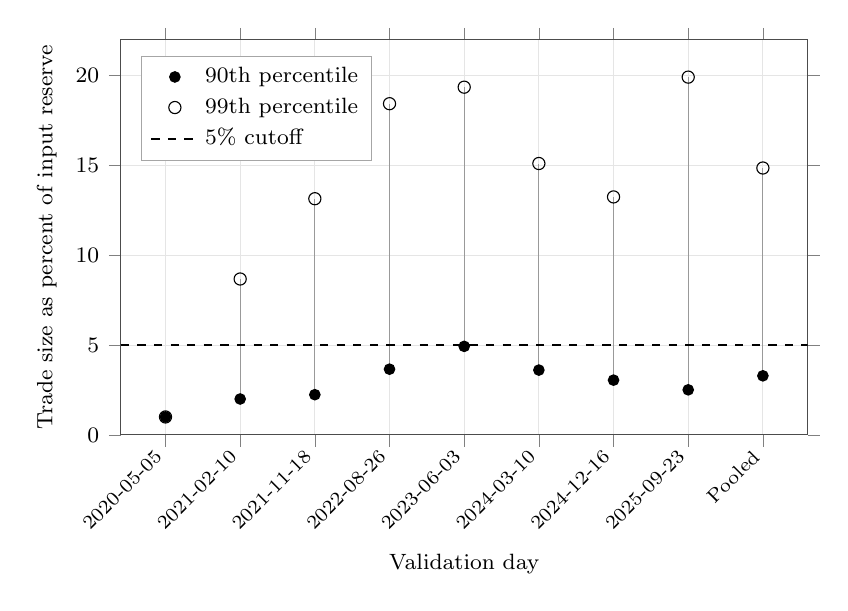
\begin{tikzpicture}
\begin{axis}[width=0.85\textwidth, height=6.6cm, xlabel={Validation day}, ylabel={Trade size as percent of input reserve}, xmin=0.4, xmax=9.6, ymin=0, ymax=22, ytick={0,5,10,15,20}, xtick={1,2,3,4,5,6,7,8,9}, xticklabels={2020-05-05,2021-02-10,2021-11-18,2022-08-26,2023-06-03,2024-03-10,2024-12-16,2025-09-23,Pooled}, x tick label style={rotate=45, anchor=east, font=\scriptsize}, tick align=outside, tick label style={font=\footnotesize}, label style={font=\footnotesize}, legend style={font=\footnotesize, draw=black!35, fill=white, at={(0.03,0.96)}, anchor=north west}, legend cell align=left, grid=major, grid style={black!10}, axis line style={black!70}]
\addplot[black!40, forget plot] coordinates {(1,1.00) (1,1.00)};
\addplot[black!40, forget plot] coordinates {(2,2.00) (2,8.68)};
\addplot[black!40, forget plot] coordinates {(3,2.24) (3,13.15)};
\addplot[black!40, forget plot] coordinates {(4,3.66) (4,18.44)};
\addplot[black!40, forget plot] coordinates {(5,4.93) (5,19.36)};
\addplot[black!40, forget plot] coordinates {(6,3.61) (6,15.11)};
\addplot[black!40, forget plot] coordinates {(7,3.05) (7,13.25)};
\addplot[black!40, forget plot] coordinates {(8,2.51) (8,19.92)};
\addplot[black!40, forget plot] coordinates {(9,3.29) (9,14.86)};
\addplot[only marks, black, mark=*, mark size=1.9pt] coordinates {(1,1.00) (2,2.00) (3,2.24) (4,3.66) (5,4.93) (6,3.61) (7,3.05) (8,2.51) (9,3.29)};
\addlegendentry{90th percentile}
\addplot[only marks, black, mark=o, mark size=2.2pt] coordinates {(1,1.00) (2,8.68) (3,13.15) (4,18.44) (5,19.36) (6,15.11) (7,13.25) (8,19.92) (9,14.86)};
\addlegendentry{99th percentile}
\addplot[black, thick, dashed, no marks] coordinates {(0.4,5) (9.6,5)};
\addlegendentry{5\% cutoff}
\end{axis}
\end{tikzpicture}
\par\vspace{6pt}
\begin{minipage}{0.92\textwidth}
\footnotesize\raggedright \emph{Notes.} The statistic is a leg's input amount as a fraction of the input-side reserve in the pool it would traverse. Points mark the 90th and 99th percentiles; the dashed line marks the 5\% cutoff. The two percentiles coincide on 2020-05-05. The sample contains 932,270 validated swaps on eight dates from 2020-05-05 through 2025-09-23.
\end{minipage}
\end{figure}
% output/exhibits/quoter_support_bounds.jsonl, per-day and pooled 90th and 99th percentiles, 932,270 validated swaps on eight sampled days

This restriction removes economically relevant observations, and the body reports that loss of support. The restriction is calibrated on executed trades, leaving the pricing error of retained hypothetical routes unobserved. A same-block closing-cycle test could provide an indirect check and remains pending.

\section{Markets omitted from the price comparison}
\label{app:coverage}

An omitted venue can improve the best direct route, the best intermediated route, or both. We therefore measure coverage using each venue's share of trading volume and report the composition of the excluded volume. To make volume comparable across the seven data sources, we compute it from individual swaps using the smaller dollar value of the two legs. This avoids double counting in two sources and removes implausible oracle values in thin pools: one Curve pool reports a \$456m day whose swaps sum to \$8, and a constant-product pair with \$255 of reserves reports \$1.36bn. Physical bounds on volume relative to reserves exclude between 0.10\% and 0.24\% of pool-days per year.
% docs/venue-coverage-bounds.md, volume reconstruction, 400 sampled days

\begin{table}[t]
\centering
\caption{Venue shares of panel volume, by year}
\label{tab:app:venues}
\begin{tabular}{lrrrrrrr}
\toprule
Year & Uni v3 & Uni v2 & Curve & Uni v4 & Balancer & Sushi v2 & Sushi v3 \\
\midrule
2020 & 0.00 & 77.51 & 11.36 & 0.00 & 0.00 & 11.13 & 0.00 \\
% docs/venue-coverage-bounds.md, seven-venue shares, sampled days in 2020
2021 & 37.97 & 31.28 & 12.25 & 0.00 & 1.18 & 17.32 & 0.00 \\
% docs/venue-coverage-bounds.md, seven-venue shares, sampled days in 2021
2022 & 64.08 & 7.01 & 18.70 & 0.00 & 5.87 & 4.35 & 0.00 \\
% docs/venue-coverage-bounds.md, seven-venue shares, sampled days in 2022
2023 & 66.81 & 9.26 & 13.88 & 0.00 & 8.80 & 1.22 & 0.03 \\
% docs/venue-coverage-bounds.md, seven-venue shares, sampled days in 2023
2024 & 69.32 & 11.67 & 12.62 & 0.00 & 5.89 & 0.49 & 0.01 \\
% docs/venue-coverage-bounds.md, seven-venue shares, sampled days in 2024
2025 & 60.14 & 4.77 & 10.96 & 22.12 & 1.69 & 0.31 & 0.01 \\
% docs/venue-coverage-bounds.md, seven-venue shares, sampled days in 2025
2026 & 49.35 & 2.43 & 13.52 & 34.24 & 0.16 & 0.12 & 0.18 \\
% docs/venue-coverage-bounds.md, seven-venue shares, sampled days in 2026
\midrule
Pooled & 56.02 & 14.98 & 13.73 & 5.45 & 3.92 & 5.88 & 0.02 \\
% docs/venue-coverage-bounds.md, pooled over all 400 sampled days
\bottomrule
\end{tabular}
\\[4pt]
\footnotesize Percentage shares within the seven-venue panel. Every seventh calendar day from 2018-11-02 to 2026-06-30, 400 sampled days.
\end{table}

Uniswap v4 carries its own within-venue limitation. Pool-identity reconstruction leaves zero swaps with incomplete or invalid immutable pool attributes across 29,005,863 rows. Static-fee pools without hooks account for 84.02\% of swaps and 99.05\% of reported value; the corresponding 2026 shares are 79.89\% and 95.57\%. The excluded remainder uses hooks, dynamic fees, or both, whose transaction-level cash-flow rule is not identified from the raw event.
% output/exhibits/v4_quote_support.jsonl, ALL and 2026 rows by support status

Curve carries between 11\% and 19\% of panel volume in every year it exists and ranks second in four years, making its coverage economically important. The StableSwap model fits 621 pool-days and excludes 588 whose 90th-percentile fitting error exceeds 1\%. Across 28 sampled dates from 2020-02-11 to 2026-04-28, these exclusions account for 34.2\% of the Curve volume assessed, or \$1.83bn of \$5.36bn. Another 2.75\% of Curve volume occurs in pool-days with too few trades to estimate and evaluate the amplification coefficient separately. Lowering the minimum from eight trades to four changes annual excluded shares by at most 1.3 percentage points.
% docs/venue-coverage-bounds.md, 28 measured pool-days from 2020-02-11 to 2026-04-28

\begin{table}[t]
\centering
\caption{Curve volume outside the StableSwap comparison}
\label{tab:app:curveleg}
\small
\begin{tabular}{lrrrrr}
\toprule
\multicolumn{6}{l}{\emph{Panel A: composition of the exclusion}} \\
Leg served & Pool-days & Volume & Of excluded & Of priced & Of that leg \\
\midrule
Native & 374 & \$1.038bn & 56.6\% & 15.7\% & 65.2\% \\
% docs/venue-coverage-bounds.md, 374 excluded Curve pool-days across 28 measured days
Stable & 119 & \$0.752bn & 41.0\% & 79.9\% & 21.1\% \\
% docs/venue-coverage-bounds.md, 119 excluded Curve pool-days across 28 measured days
Other volatile & 95 & \$0.045bn & 2.4\% & 4.4\% & 22.2\% \\
% docs/venue-coverage-bounds.md, 95 excluded Curve pool-days across 28 measured days
\midrule
\multicolumn{6}{l}{\emph{Panel B: excluded share of each leg's volume, by year}} \\
Year & \multicolumn{2}{r}{Native leg} & \multicolumn{2}{r}{Stable leg} & Other volatile \\
\midrule
2021 & \multicolumn{2}{r}{85.49\%} & \multicolumn{2}{r}{46.91\%} & 15.23\% \\
% docs/venue-coverage-bounds.md, Curve pool-days sampled in 2021
2022 & \multicolumn{2}{r}{68.82\%} & \multicolumn{2}{r}{30.21\%} & 50.77\% \\
% docs/venue-coverage-bounds.md, Curve pool-days sampled in 2022
2023 & \multicolumn{2}{r}{59.11\%} & \multicolumn{2}{r}{5.51\%} & 56.60\% \\
% docs/venue-coverage-bounds.md, Curve pool-days sampled in 2023
2024 & \multicolumn{2}{r}{48.24\%} & \multicolumn{2}{r}{0.94\%} & 14.38\% \\
% docs/venue-coverage-bounds.md, Curve pool-days sampled in 2024
2025 & \multicolumn{2}{r}{47.47\%} & \multicolumn{2}{r}{13.96\%} & 10.52\% \\
% docs/venue-coverage-bounds.md, Curve pool-days sampled in 2025
2026 & \multicolumn{2}{r}{60.92\%} & \multicolumn{2}{r}{9.04\%} & 20.08\% \\
% docs/venue-coverage-bounds.md, Curve pool-days sampled in 2026
\bottomrule
\end{tabular}
\\[4pt]
\footnotesize A pool serves the \emph{native} leg when it contains ETH or a staking derivative, the \emph{stable} leg when every token is stable including baskets and interest-bearing wrappers, and the \emph{other volatile} leg otherwise. The sample contains 28 measured Curve pool-days from 2020-02-11 to 2026-04-28. Pool leg is assigned by a token registry pass followed by a symbol pass over stable derivatives, which is required because the registry alone labels metapools pairing a stablecoin against the three-token base-pool claim as volatile pairs.
\end{table}

The exclusions are concentrated in routes involving the native asset. The excluded share of native-leg volume exceeds the stable-leg share by at least 33 percentage points in every sample year and by 54 points in 2023. Tricrypto pools pairing WBTC and WETH with a stablecoin account for \$818m, or 44.6\%, of the \$1.83bn excluded, including seven of the twelve largest excluded pool-days. These pools use CryptoSwap, so the missing coverage is concentrated where Curve supplies depth between ETH and stablecoins.
% docs/venue-coverage-bounds.md, curve_excluded_composition.jsonl, 28 measured pool-days

SushiSwap v3 cannot be priced from the available historical records. Its reserves are distributed across ticks, but the source omits \texttt{sqrtPriceX96}, in-range liquidity, and tick spacing. The balance and weight fields exposed by the common schema do not describe its concentrated-liquidity invariant. This omission is quantitatively small: the venue accounts for 0.016\% of priced-venue volume over the full sample and 0.176\% in 2026. Across fourteen sampled days, only 4.1\% of its volume occurs on token pairs unavailable on another priced venue, never more than \$37,609 on one day.
% docs/venue-coverage-bounds.md, sushiswap_v3_schema_probe.jsonl and sushiswap_v3_pair_overlap.jsonl, 14 sampled days

Balancer accounts for 3.9\% of measured venue volume over the full sample and 8.8\% at its 2023 peak. Weighted pools are included with the validation errors in Table~\ref{tab:app:weighted}. Linear and boosted pools remain outside the comparison. Of 29 sampled composable-stable pools, 23 reduce to two external tokens after removing the pool's own share token, but pricing them also requires historical rate-provider states that are not available in the current source.
% docs/venue-coverage-bounds.md, venue_volume_by_year.jsonl, 400 sampled days; docs/research-workflow.md, Balancer family audit

\section{Round-trip exclusion}
\label{app:roundtrip}

A route whose first input token equals its last output token,
\[
\mathbf{1}\{\,a_{\mathrm{first}} = b_{\mathrm{last}}\,\},
\]
does not represent endpoint-to-endpoint conversion under the paper's route unit. Such routes are removed everywhere before anything is measured because they would otherwise enter a routing statistic as though a trader had chosen an intermediary between distinct endpoints. The excluded population can contain cyclic arbitrage and other self-returning activity; the endpoint rule does not label every route as arbitrage or wash trading. Multi-trade arbitrage can be bundled atomically \citep{DaianEtAl2020FlashBoys}, which supports the mechanism but not an exhaustive behavioural classification.

\begin{table}[t]
\centering
\caption{Round-trip share of multi-leg routing, across 79 sampled days}
\label{tab:app:roundtrip}
\begin{tabular}{lrr}
\toprule
Quantile across days & Share by count & Share by value \\
\midrule
Minimum & 4.45\% & 7.40\% \\
% output/exhibits/round_trip_share_by_day.jsonl, 79 sampled days, minima on 2020-06-01 and 2023-04-03
25th percentile & 9.60\% & 17.73\% \\
% output/exhibits/round_trip_share_by_day.jsonl, 79 sampled days
Median & 12.70\% & 21.72\% \\
% output/exhibits/round_trip_share_by_day.jsonl, 79 sampled days
75th percentile & 17.04\% & 29.56\% \\
% output/exhibits/round_trip_share_by_day.jsonl, 79 sampled days
90th percentile & 20.03\% & 46.11\% \\
% output/exhibits/round_trip_share_by_day.jsonl, 79 sampled days
Maximum & 25.93\% & 91.31\% \\
% output/exhibits/round_trip_share_by_day.jsonl, 79 sampled days, both maxima on 2025-12-06
\midrule
2020 median & 11.77\% & 14.08\% \\
% output/exhibits/round_trip_share_by_day.jsonl, 8 sampled days in 2020
2021 median & 13.21\% & 25.35\% \\
% output/exhibits/round_trip_share_by_day.jsonl, 13 sampled days in 2021
2022 median & 16.72\% & 21.89\% \\
% output/exhibits/round_trip_share_by_day.jsonl, 13 sampled days in 2022
2023 median & 8.51\% & 17.71\% \\
% output/exhibits/round_trip_share_by_day.jsonl, 13 sampled days in 2023
2024 median & 9.60\% & 21.13\% \\
% output/exhibits/round_trip_share_by_day.jsonl, 13 sampled days in 2024
2025 median & 16.75\% & 36.08\% \\
% output/exhibits/round_trip_share_by_day.jsonl, 14 sampled days in 2025
2026 median & 20.80\% & 20.32\% \\
% output/exhibits/round_trip_share_by_day.jsonl, 5 sampled days in 2026
\bottomrule
\end{tabular}
\\[4pt]
\footnotesize Round trips as a share of multi-leg routes. The sample contains 79 dates from 2020-06-01 through 2026-04-27 and 13,160,047 routes, of which 2,488,399 are multi-leg and 351,553 are round trips. Dates with fewer than 200 multi-leg routes are omitted.
\end{table}

The value-weighted share exceeds the count-weighted share at every quantile, by a factor between 1.7 and 3.5, which is consistent with large atomic cycles sitting inside a much larger population of smaller routes. No sampled day is free of them, and the floor of 4.45\% by count falls on 2020-06-01, the earliest day sampled. Count-weighting is used throughout the body because a value-weighted routing statistic on an unscreened panel would give disproportionate influence to this self-returning population. Figure~\ref{fig:app:roundtrip} plots both shares for every sampled day, with the two medians and the extreme day marked.
% output/exhibits/round_trip_share_by_day.jsonl, 79 sampled days from 2020-06-01 to 2026-04-27

\begin{figure}[tbp]
\centering
\caption{Round-trip contamination of multi-leg routing, day by day}
\label{fig:app:roundtrip}
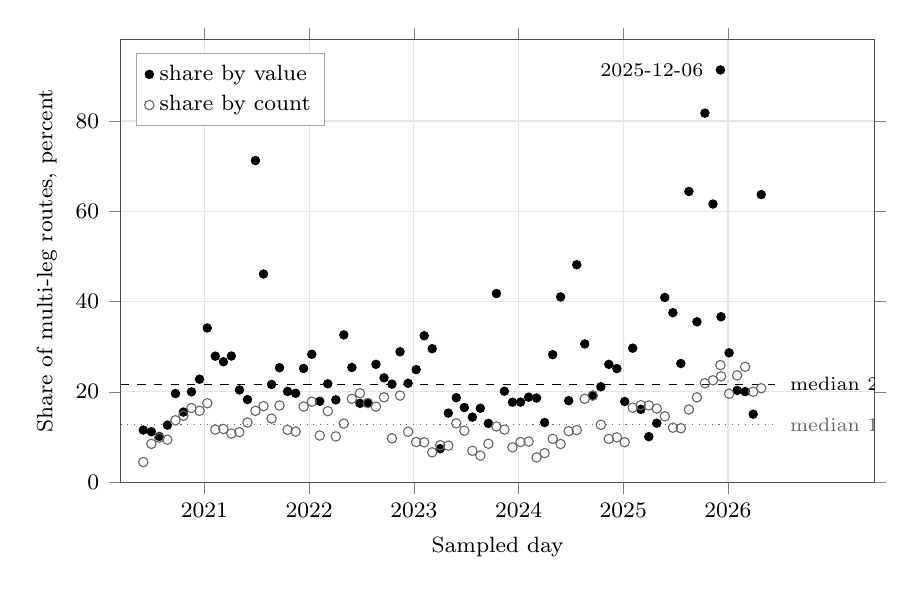
\begin{tikzpicture}
\begin{axis}[width=0.92\textwidth, height=7.2cm, xlabel={Sampled day}, ylabel={Share of multi-leg routes, percent}, xmin=2020.2, xmax=2027.4, ymin=0, ymax=98, xtick={2021,2022,2023,2024,2025,2026}, xticklabel style={/pgf/number format/1000 sep={}}, ytick={0,20,40,60,80}, tick align=outside, tick label style={font=\footnotesize}, label style={font=\footnotesize}, legend style={font=\footnotesize, draw=black!35, fill=white, at={(0.02,0.97)}, anchor=north west}, legend cell align=left, grid=major, grid style={black!10}, axis line style={black!70}]
\addplot[only marks, black, mark=*, mark size=1.5pt] coordinates {(2020.416,11.54) (2020.493,11.17) (2020.569,10.12) (2020.646,12.63) (2020.723,19.62) (2020.799,15.52) (2020.876,20.01) (2020.953,22.80) (2021.027,34.15) (2021.104,27.91) (2021.181,26.67) (2021.257,27.94) (2021.334,20.43) (2021.411,18.29) (2021.487,71.24) (2021.564,46.11) (2021.641,21.64) (2021.717,25.35) (2021.794,20.09) (2021.871,19.68) (2021.947,25.18) (2022.025,28.33) (2022.101,17.92) (2022.178,21.79) (2022.255,18.23) (2022.331,32.62) (2022.408,25.40) (2022.485,17.46) (2022.561,17.57) (2022.638,26.10) (2022.715,23.11) (2022.791,21.72) (2022.868,28.88) (2022.945,21.89) (2023.022,24.93) (2023.099,32.43) (2023.175,29.56) (2023.252,7.40) (2023.329,15.30) (2023.405,18.70) (2023.482,16.53) (2023.559,14.40) (2023.635,16.37) (2023.712,13.02) (2023.789,41.78) (2023.865,20.14) (2023.942,17.71) (2024.019,17.73) (2024.096,18.82) (2024.172,18.63) (2024.249,13.20) (2024.326,28.25) (2024.402,41.03) (2024.479,18.05) (2024.556,48.16) (2024.632,30.62) (2024.709,19.25) (2024.786,21.13) (2024.862,26.10) (2024.939,25.16) (2025.014,17.86) (2025.090,29.68) (2025.167,16.14) (2025.244,10.08) (2025.320,13.06) (2025.397,40.91) (2025.474,37.54) (2025.550,26.28) (2025.627,64.39) (2025.704,35.52) (2025.780,81.75) (2025.857,61.61) (2025.928,91.31) (2025.934,36.64) (2026.011,28.65) (2026.088,20.32) (2026.164,20.06) (2026.241,15.06) (2026.318,63.70)};
\addlegendentry{share by value}
\addplot[only marks, black!60, mark=o, mark size=1.7pt] coordinates {(2020.416,4.45) (2020.493,8.49) (2020.569,9.83) (2020.646,9.41) (2020.723,13.70) (2020.799,14.72) (2020.876,16.42) (2020.953,15.81) (2021.027,17.48) (2021.104,11.64) (2021.181,11.77) (2021.257,10.76) (2021.334,11.07) (2021.411,13.21) (2021.487,15.79) (2021.564,16.84) (2021.641,14.08) (2021.717,16.98) (2021.794,11.57) (2021.871,11.19) (2021.947,16.75) (2022.025,17.82) (2022.101,10.33) (2022.178,15.72) (2022.255,10.13) (2022.331,12.96) (2022.408,18.46) (2022.485,19.69) (2022.561,17.53) (2022.638,16.72) (2022.715,18.80) (2022.791,9.71) (2022.868,19.18) (2022.945,11.17) (2023.022,8.89) (2023.099,8.82) (2023.175,6.60) (2023.252,8.18) (2023.329,8.09) (2023.405,13.02) (2023.482,11.40) (2023.559,6.94) (2023.635,5.88) (2023.712,8.51) (2023.789,12.33) (2023.865,11.64) (2023.942,7.70) (2024.019,8.89) (2024.096,9.00) (2024.172,5.47) (2024.249,6.44) (2024.326,9.60) (2024.402,8.45) (2024.479,11.29) (2024.556,11.53) (2024.632,18.46) (2024.709,19.17) (2024.786,12.70) (2024.862,9.58) (2024.939,9.92) (2025.014,8.85) (2025.090,16.50) (2025.167,17.04) (2025.244,17.00) (2025.320,16.29) (2025.397,14.59) (2025.474,12.06) (2025.550,11.94) (2025.627,16.09) (2025.704,18.79) (2025.780,21.91) (2025.857,22.56) (2025.928,25.93) (2025.934,23.44) (2026.011,19.58) (2026.088,23.65) (2026.164,25.55) (2026.241,20.03) (2026.318,20.80)};
\addlegendentry{share by count}
\addplot[black, dashed, thin, no marks, forget plot] coordinates {(2020.2,21.72) (2026.45,21.72)};
\addplot[black!60, dotted, thin, no marks, forget plot] coordinates {(2020.2,12.70) (2026.45,12.70)};
\node[anchor=west, font=\scriptsize] at (axis cs:2026.5,21.72) {median 21.7};
\node[anchor=west, font=\scriptsize, black!60] at (axis cs:2026.5,12.70) {median 12.7};
\node[anchor=east, font=\scriptsize] at (axis cs:2025.86,91.31) {2025-12-06};
\end{axis}
\end{tikzpicture}
\par\vspace{6pt}
\begin{minipage}{0.92\textwidth}
\footnotesize\raggedright \emph{Notes.} Each mark is one sampled date. \emph{Share by value} weights round-trip routes by their notional; \emph{share by count} gives each route equal weight. Both shares use multi-leg routes as the denominator. Dashed and dotted lines mark the respective medians, and the highest point is labelled. Dates with fewer than 200 multi-leg routes are omitted. The sample contains 79 dates from 2020-06-01 through 2026-04-27 and 2,488,399 multi-leg routes.
\end{minipage}
\end{figure}
% output/exhibits/round_trip_share_by_day.jsonl, share_by_count and share_by_value on 79 sampled days from 2020-06-01 to 2026-04-27
